\chapter{Design}
\label{ch:Design}

\section{Theoretische Grundlagen}

Zunächst sollen die grundlegenden Eigenschaften der erwarteten Eingangssignale definiert und näher beschrieben werden. 

\subsection{Zeit- und wertdiskrete digitale Signale}

Bei den Eingangssignalen des Event-Recorders handelt es sich um die Ausgänge von Mikrocontrollern oder anderer digitaler Schaltungen und damit um digitale Signal.
Digitale Signale sind durch zwei grundlegende Eigenschaften charakterisiert, sie sind:
\begin{itemize}
	\item \textbf{zeitdiskret}, und
	\item \textbf{wertdiskret}
\end{itemize}
\textbf{Wertdiskret} bedeutet, dass das Signal nur genau einen Wert aus einer festgelegten Anzahl möglicher Wertezustände annehmen kann.
In den meisten Fällen beschränkt sich der Wertebereich auf die Binärwerte ``1'' oder ``0'', das heißt ein digitales Signal ist zum Beispiel bei 0,1 Volt Spannung ``0'' und bei 3,2 Volt ``1'', wohingegen ein analoges Signal alle möglichen Werte zwischen 0 und 3,3 Volt annehmen kann.\\

\textbf{Zeitdiskret} bedeutet, dass ein digitales Signal ``nur zu bestimmten periodischen Zeitpunkten definiert ist bzw. nur dann eine Veränderung im Signalwert aufweist''\cite{wiki:Digitalsignal}, das heißt dass das Signal bei der Erfassung mit einem festen ``Zeitraster'' abgetastet wird und zwischen den Rasterpunkten einen festen Wert behält.

Bei der Erfassung digitaler Signale ist es nötig, dass die Abtastfrequenz nach Nyquist-Shannon-Abtasttheorem mindestens doppelt so hoch als die maximale Frequenz des untersuchten Signals sein muss, damit keine Informationen aus dem Ausgangsignal verloren gehen (vgl. \cite{wiki:Digitalsignal}).

Es ist zu beachten, dass es sich bei der Definition von digitalen Signalen um eine idealisierte Ansicht handelt und dass sich bei realen digitalen Signale oft -- vor allem bei hohen Frequenzen -- Störeffekte zeigen. Ein Beispiel für einen Störeffekt wäre das ``Prellen'' eines mechanischen Schalters, bei dem es durch den mechanischen Kontakt zu einem mehrfachen Signalwechsel kommen kann, bevor ein stabiles Signal anliegt. Wenn der Schalter-Zustand dabei mit vergleichsweise langsamer Geschwindigkeit ausgelesen wird, gehen die deutlich schnelleren Signalwechsel gemäß dem Nyquist-Shannon-Abstasttheorem nicht in das Ausgangssignal ein, bei entsprechend hoher Abtastrate werden sie allerdins mit in Ausgangssignal übernommen und können dann unerwünschte Effekte auslösen.\\
Bei der in dieser Arbeit verwendeten Hardware sind keine speziellen Vorrichtungen (wie zum Beispiel ``Schmitt-Trigger'') vorhanden um solchen Effekten entgegen zu wirken, das heißt es wird am Eingang ein für die Analyse aussreichend stabiles Signal erwartet.   \\

Damit die Ergebnisse des Event-Recorders richtig auswertet werden können, muss zu jeder Signaländerung der ``diskrete'' Zeitpunkt bekannt sein, das heißt das Zeitraster der Abtastung muss numeriert werden, so dass jeder Signaländerung ein eindeutiger Zeitstempel zugeordnet werden kann.
Diese ``Numerierung'' wird umgesetzt, in dem der von einem Oszillator\footnote{Eigener Hardware-Baustein, der eine konstant auf- und abschwingende Spannung erzeugt und damit zur Taktung digitaler Schaltung verwendet werden kann} generierte Schaltungstakt mit einer Zählerschaltung aufaddiert wird. Der Zeitstempel entspricht dann einfach dem aktuellen Zählerstand.\\


\begin{table}[h]
\centering
\begin{tabular}{|l|l|l|}
\hline
\rowcolor[HTML]{EFEFEF} 
	EVENT\_ID [8 Bit] & INPUT\_DATA [8 Bit] & TIMESTAMP [16 Bit]\\ \hline
	\multicolumn{1}{|c|}{0x02} & \multicolumn{1}{c|}{0x01} & \multicolumn{1}{c|}{0x0EF8} \\ \hline
\end{tabular}
\caption{Beispielhafte Darstellung eines aufgenommenen Events mit 16-Bit Zeitstempel}
\label{my-label}
\end{table}


Die Bit-Breite des Zählers legt zusammen mit der Geschwindigkeit des Takts die maximal mögliche Aufnahmelänge fest. Der verwendete Zähler hat eine Breite von 46 Bit, womit sich bei einer Taktfrequenz von 100 Mhz zum Beispiel eine Laufzeit von ca. 195 Stunden ergibt\footnote{Berechnung: \(2^{46} * \frac{1}{100 Mhz} = 2^{47} * 10 ns\) } (was für die meisten Anwendungsfälle mehr als aussreichend ist). 



\subsection{Definition ``Event''}

Für diese Arbeit soll unter dem Begriff ``Event'' ein vom Benutzer festgelegter Signalzustand oder eine Signaländerung an den Eingangspins des Event-Recorders verstanden werden. In den meisten Fällen macht es mehr Sinn eine Signaländerung zu definieren, als einen Zustand, da bei einem anhaltenden Zustand auch das Event kontinuierlich ``ausgelöst'' wird, und ein dementsprechend hohes Datenvolumen erzeugt.\\
Es ergeben sich folgende Definitionsmöglichkeiten für die einzelnen Eingangs-Pins:
\begin{itemize}
	\item ``0'': niedriger logischer Pegel
	\item ``1'': hoher logischer Pegel
	\item ``u'': steigender Pegel
	\item ``d'': fallender Pegel
	\item ``x'': beliebiger Zustand ("don't care") 
\end{itemize}
Zusätzlich wäre eine Kombination von ``u'' und ``d'' denkbar, die auf beliebige Signaländerungen reagiert.
Eine Verkettung dieser Möglichkeiten bei der jedem Eingangspins ein Zustand zugewiesen wird soll als ``Event-Trigger'' -- also als Auslöser eines bestimmten Events -- bezeichnet werden.\\
Dies entspricht im Wesentlichen der Definition von \textit{Trigger} die bei ``traditionellen'' Logikanalysatoren verwendet wird, allerdings mit dem Unterschied dass der Trigger bei einem ``traditionellen'' Logikanalysator die eigentliche Aufnahme einmalig auslöst, und dann bis zum Ende der Aufnahme nicht mehr von Bedeutung ist, während ein Event-Trigger als Teil der Aufnahme kontinuierlich überprüft werden muss und erst bei Erfüllung der Triggerbedingung überhaupt Ausgangsdaten generiert werden.\\
Es bietet sich an einem Event zusätzlich bestimme Funktionen zuweisen zu können, wie zum Beispiel das Starten\footnote{Die Erkennung eines Start-Events erfordet folglich, dass auch im ``Ruhezustand'' eine Event-Erkennung durchgeführt wird} und Stoppen der Event-Erkennung, oder das Wechseln in einen zusätzlichen Modus, bei dem auf alle Signaländerungen reagiert wird.\\
Wie in der Einführung erwähnt soll die Definition der Events in Text-Form möglich sein und kann dann z.B. folgendermaßen aussehen:

\begin{lstlisting}[language=yaml]
# event configuration
events: 
  - start:
          trigger: uxxxxxxx
          func: start

  - stop:
          trigger: dxxxxxxx
          func: stop

  - event1:
          trigger: 1uxxxxxx

  - event2:
          trigger: 1xuxxxxx
          func: dump_begin
...
\end{lstlisting}

\clearpage
\section{Überblick der benötigten Hard- und Software-Komponenten}
\subsection{Datenerfassung: FPGA}
Wie im vorherigen Kapitel beschrieben wird für die Datenerfassung eine Zählerschaltung benötigt, die einen stabilen Zeitstempel liefern kann. Vorraussetzung dafür ist, dass der Zähler kontinuierlich läuft und nicht durch andere Vorgänge unterbrochen werden kann. Dies ist bei PC-Systemen oder auch Mikrocontrollern nicht ohne weiteres möglich, da die Programmausführung zu jedem Zeitpunkt von Betriebssystem-Funktionen oder Interrupt-Routinen\footnote{Bei einer Interrupt-Routine wird die aktuelle Programmausführung auf CPU-Ebene pausiert, zum Beispiel um auf Ereignisse externer Hardwaregeräte reagieren zu können} pausiert werden kann.\\
Deswegen bietet sich hier die Verwendung einer programmierbaren logischen Schaltung wie zum Beispiel eines CPLDs (\acrlong{CPLD}) oder FPGAs (\acrlong{FPGA}) an, bei dem eine von anderen Komponenten vollkommen unabhängige parallele Ausführung des Zählers möglich ist.\\
Sowohl CPLD- als auch FPGA-Chips bestehen aus einer Vielzahl von einheitlichen Blöcken (``PLBs'') die einfache logische Funktionen abbilden können. Im Vergleich zu logischen Gattern sind die die Blöcke in ihrer Funktion aber frei konfigurierbar. Durch die Vernetzung der so konfigurierten Blöcke können umfangreiche digitale Schaltungen realisiert werden.\\
FPGAs sind etwas komplexer aufgebaut als CPLDs, dabei aber auch flexibler bei der Vernetzung und enthalten oft zusätzliche Funktionsblöcke wie den in der nachfolgenden Abbildung erkennbaren Block-RAM als Zwischenspeicher für größere Datenmengen oder die \acrshort{PLL}-Einheit zur Erzeugung von Taktsignalen mit konfigurierbarer Geschwindigkeit (vgl. \cite{wiki:PLD}).

\begin{figure}[htbp]
	\centering
		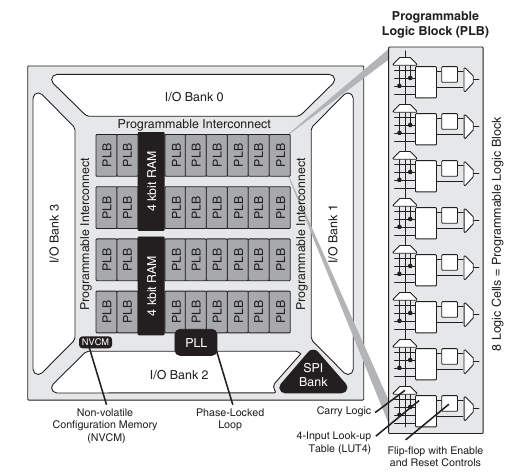
\includegraphics[width=0.80\textwidth]{../figures/iCE40_block_diagram.png}
	\caption[Blockdiagramm des verwendeten iCE40 FPGAs]{Aufbau des verwendeten iCE40 FPGAs (Quelle: iCE40 Datasheet{\cite{doc:datasheet}})}
	\label{fig:ice40_block_diagram}
\end{figure}

Zusätzlich ist die Anzahl von Funktionsblöcken bei FPGAs üblicherweise deutlich höher als als bei CPLDs, weswegen in dieser Arbeit ein FPGA-Chip verwendet werden soll.

Die in der Abbildung erkennbaren I/O-Bänke beinhalten GPIO-Pins die als Ein- oder Ausgänge konfiguriert und direkt mit den Logikblöcken (``PLBs'') im FPGA verknüpft werden können.

\subsection{Datenzwischenspeicher: SRAM}

Nach der Erfassung müssen die Daten zwischengespeichert werden. Dabei sind vor allem zwei Faktoren entscheidend:
\begin{itemize} 
	\item Die \textbf{Geschwindigkeit} des Speichers, die meist den maximalen Datendurchsatz der Gesamtschaltung bestimmt
	\item Die \textbf{Größe} des Speichers, die festlegt wie lange bei hohem Datendatendurchsatz aufgenommen werden kann 
\end{itemize}
Die meisten nicht-flüchtigen Speicher sind aufgrund der unzureichenden Geschwindigkeit nicht für diesen Anwendungszweck geeignet, weswegen sich die Verwendung von \acrshort{RAM}-Speicher anbietet. \\
Bei Mikrocontrollern und kleineren FPGA-Boards werden aus Kostengründen und wegen der unkomplizierten Ansteuerung oft SRAM-Speichereinheiten verbaut. SRAM-Speicher hat meist sehr kurze Zugriffszeiten, allerdings bei einer geringen Speichergröße von wenigen MBit. Der in dieser Arbeit verwendete SRAM-Speicher hat beispielsweise eine Größe von 4 Mbit (512 KB) und könnte damit 62500 Events zwischenspeichern\footnote{Bei einer angenommenen Event-Größe von 64-Bit, und unter der Annahme dass der SRAM-Speicher ausschließlich zum Zwischenspeichern von Events verdwendet wird}.\\
Bei kontinuierlicher Erfassungs mit einer Abtastrate von 100 Mhz entspricht dies einer Aufnahmezeit von unter einer Millisekunde\footnote{$62500 * 10 ns = 0.625 ms$}. Da allerdings keine Eingangssignale erwartet werden, bei denen Events mit einer Frequenz von 100 Mhz auftreten und außerdem bereits bei laufender Aufnahme Events aus dem RAM-Speicher entnommen und weiter übertragen werden, kann der SRAM-Speicher trotzdem im Sinne der Aufgabenstellung als Zwischenspeicher verwendet werden.\\
Als Alternative könnte DRAM-Speicher verwendet werden, der ein Vielfaches der Speichergröße bietet und damit auch längere Aufnahmen bei hoher Signaldichte ermöglichen würde. DRAM-Speicher erfordert allerdings im Vergleich zu SRAM ein kontinuierliches ``Auffrischen'' der Speicher-Inhalte durch eine Controller-Einheit und bedeutet deshalb deutlich mehr Aufwand bei der Implementierung.


\subsection{Datenübertragung: SPI}

Nach der Datenerfassung und Zwischenspeicherung werden die Daten an ein externes System übertragen, an dem sie weiterverarbeitet oder ausgewertet werden können. Zur Datenübertragung gibt es eine Vielzahl von Schnittstellen und Protokollen. Dabei werden die Daten im Normalfall ``serialisiert'', das heißt wenn ein Event aus 64 Bit besteht, werden die Bits nacheinander über eine einzige Datenleitung übertragen. Geläufige serielle Datenübertragungsverfahren sind vor allem \acrshort{UART}, \acrshort{I2C} und \acrshort{SPI}.
\begin{description}
	\item Bei einem \textbf{UART (\acrlong{UART})} werden die Daten über eine Empfangs- und eine Sendeleitung ausgetauscht. Es wird kein eigenes Taktsignal übertragen, weswegen auf beiden Seiten eine feste Übertragungsgeschwindigkeit (``Baud-Rate'') eingestellt werden muss. UART-Schnittstellen sind weit verbreitet, bei üblichen Baud-Raten ist die Übetragungsgeschwindigkeit allerdings relaitv gering (vgl. \cite{wiki:UART}).
	\item \textbf{\acrshort{I2C} (\acrlong{I2C})} ist ein synchroner Datenbus, bei dem eine eigene Leitung für den Takt und eine Datenleitung verwendet wird. $\text{I}^2$C arbeitet nach dem Master-Slave-Prinzip, das heißt es können auch mehrere Geräte miteinander kommunizieren. $\text{I}^2$C untertützt Übertragungsraten bis zu 5 Mbit/s (unidirektional, vgl. \cite{wiki:I2C}).
	\item \textbf{\acrshort{SPI} (\acrlong{SPI})} ist wie $\text{I}^2$C ein synchroner Datenbus nach dem Master-Slave-Prinzip. Neben der Leitung für den Takt wird eine Daten-Leitung in Senderichtung und eine Datenleitung in Empfangsrichtung verwendet. Zusätzlich wird pro Gerät eine ``Chip-Select'' Leitung benötigt, um die Geräte adressieren zu können. SPI kann Übertragungsraten bis in den mehrstelligen Megabit-Bereich ermöglichen (vgl. \cite{wiki:SPI}).
\end{description}

Aufgrund der hohen Übertragungsrate und der relativ unkomplizierten Implementierungsmöglichkeiten soll SPI für die Datenübetragung verwendet werden.


\subsection{Steuerung der Aufnahme und sequentielle Programmabläufe}

Neben der reinen Datenerfassung und -Übertragung werden noch Komponenten zur Steuerung und zur Kontrolle des Aufnahmevorgangs benötigt.\\
Grundsätzlich können die benötigten Vorgänge- und Zustände (zum Beispiel das Starten und Stoppen der Aufnahme) direkt im FPGA umgesetzt werden. Als Kommunikationsweg zur Steuerung und Konfiguration kann dann wiederum SPI verwendet werden.\\
Bei längeren oder komplexeren Programmabläufen die keine zeitkritische Ausführung erfordern bietet sich die Verwendung eines zusätzlichen Mikrocontrollers an. Da die meisten PC-Systeme keine programmierbaren \acrshort{GPIO}-Pins als SPI-Schnittstelle zur Verfügung stellen, kann ein Mikrocontroller außerdem als Brücke zwischen FPGA und Anwendersystem fungieren, und zum Beispiel die vom FPGA erfassten Daten über einen USB-Port zur Verfügung stellen.\\
Davon abgesehen wird auch auch die entsprechende Hardware- und Software-Infrstruktur benötig um das FPGA und den Mikrokonroller zu programmieren und zu konfigieren.
\clearpage

\section{Auswahl der Software-Toolchain: IceStorm}
\clearpage

\section{Auswahl der Hardware}

\subsection{IceZero FPGA-Shield (iCE40HX4K)}
FPGA: iCE40
vielzahl boards:
	z.B. https://embeddedmicro.com/products/mojo-v3
	-> SDRAM

	-> keine Opensource-Toolchain!

iCE40:
	erst:
	https://www.olimex.com/Products/FPGA/iCE40/iCE40HX1K-EVB/open-source-hardware

	dann icezero:

	- formfaktor


\subsection{Raspberry Pi Zero W}

Controller:
	pi: preis, vielfältigkeit, formfaktor

\clearpage

\section{Beispiel: Von der Synthese bis zum Bitstream mit der IceStorm-Toolchain}
\clearpage


